% !Mode:: "TeX:UTF-8"
% !TEX encoding = UTF-8 Unicode

\begin{center}
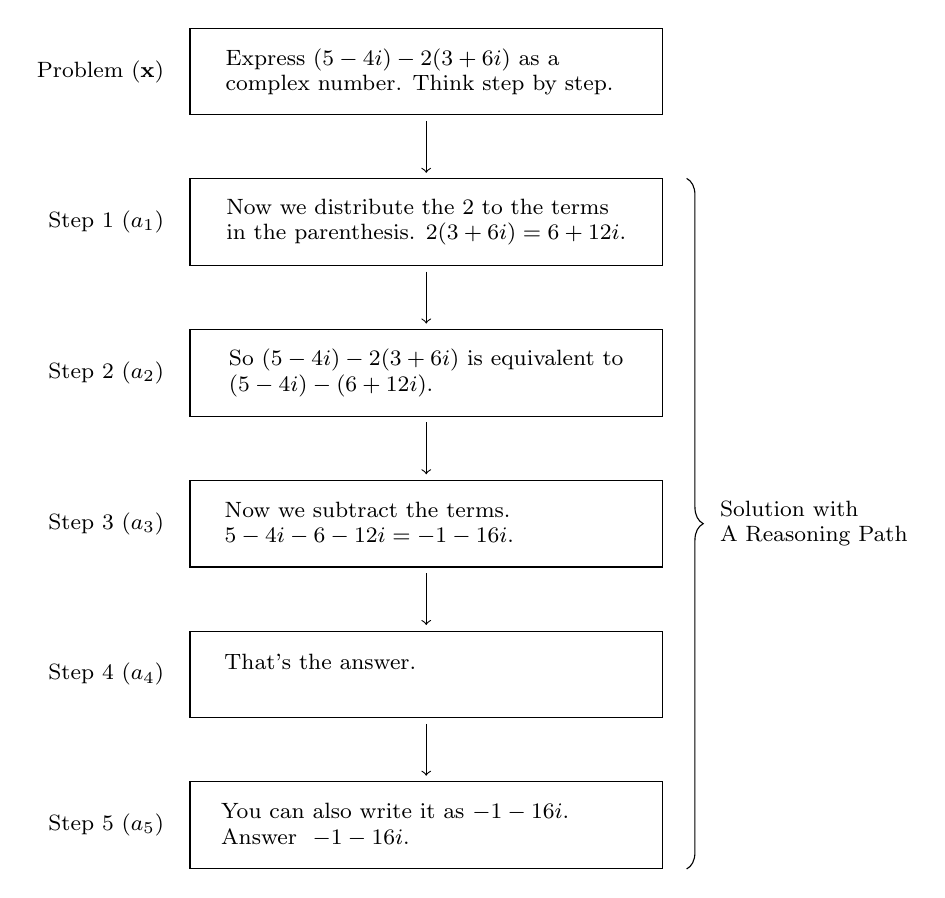
\begin{tikzpicture}
	
\def\ssep{0.1cm}
\def\bsep{2.5cm}

\tikzstyle{snode} = [minimum width=0.8cm,minimum height=0.5cm,inner sep=1pt,draw,thin];
\tikzstyle{rnode} = [minimum width=6cm,minimum height=1.1cm,inner sep=2pt,draw];

\begin{scope}

\node [rnode,anchor=west,align=left] (x) at (0,0) {\footnotesize{Express $(5-4i)-2(3+6i)$ as a \hspace{0.60cm}{\color{white} x}}\\[-0.1cm] \footnotesize{complex number. Think step by step.}};

\node [rnode,anchor=north west,align=left] (step1) at ([yshift=-0.8cm]x.south west) {\footnotesize{Now we distribute the $2$ to the terms}\\[-0.1cm] \footnotesize{in the parenthesis. $2(3+6i) = 6+12i$.}};

\node [rnode,anchor=north west,align=left] (step2) at ([yshift=-0.8cm]step1.south west) {\footnotesize{So $(5-4i)-2(3+6i)$ is equivalent to}\\[-0.1cm] \footnotesize{$(5-4i)-(6+12i)$.}};

\node [rnode,anchor=north west,align=left] (step3) at ([yshift=-0.8cm]step2.south west) {\footnotesize{Now we subtract the terms. \hspace{1.2cm}{\color{white} x}}\\[-0.1cm] \footnotesize{$5-4i-6-12i = -1-16i$.}};

\node [rnode,anchor=north west,align=left] (step4) at ([yshift=-0.8cm]step3.south west) {\footnotesize{That's the answer. \hspace{2.4cm}{\color{white} x}}\\[-0.1cm] \footnotesize{}};

\node [rnode,anchor=north west,align=left] (step5) at ([yshift=-0.8cm]step4.south west) {\footnotesize{You can also write it as $-1-16i$. \hspace{0.5cm}{\color{white} x}}\\[-0.1cm] \footnotesize{Answer\ \ $-1-16i$.}};

\draw [->] ([yshift=-2pt]x.south) -- ([yshift=2pt]step1.north);
\draw [->] ([yshift=-2pt]step1.south) -- ([yshift=2pt]step2.north);
\draw [->] ([yshift=-2pt]step2.south) -- ([yshift=2pt]step3.north);
\draw [->] ([yshift=-2pt]step3.south) -- ([yshift=2pt]step4.north);
\draw [->] ([yshift=-2pt]step4.south) -- ([yshift=2pt]step5.north);

\node [anchor=east] (xlabel) at ([xshift=-0.2cm]x.west) {\footnotesize{Problem ($\mathbf{x}$)}};
\node [anchor=east] (step1label) at ([xshift=-0.2cm]step1.west) {\footnotesize{Step 1 ($a_1$)}};
\node [anchor=east] (step2label) at ([xshift=-0.2cm]step2.west) {\footnotesize{Step 2 ($a_2$)}};
\node [anchor=east] (step3label) at ([xshift=-0.2cm]step3.west) {\footnotesize{Step 3 ($a_3$)}};
\node [anchor=east] (step4label) at ([xshift=-0.2cm]step4.west) {\footnotesize{Step 4 ($a_4$)}};
\node [anchor=east] (step5label) at ([xshift=-0.2cm]step5.west) {\footnotesize{Step 5 ($a_5$)}};

\draw [decoration={brace,amplitude=6pt},decorate] ([yshift=0.0cm,xshift=0.3cm]step1.north east) -- ([yshift=0.0cm,xshift=0.3cm]step5.south east) node [right,pos=0.5,xshift=0.3cm,align=left] {\footnotesize{Solution with}\\[-0.1cm] \footnotesize{A Reasoning Path}};


\end{scope}

\end{tikzpicture}
\end{center}
